%% stevensthesis_num.tex
%% Copyright 2008 B. E. Arnett
%
% ----->  Latex is not required for writing your dissertation or thesis.  Most theses in liberal arts and other areas are done in Word or WYSIWYG editors
%------>  Latex is frequently used in math, physics and computer science for ease in producing formulas.  
%------>  This template is provided for Latex users to help in the formatting of the thesis or dissertation.  
%------>  This work is not maintained by Stevens Library anymore and is provided on an: "as is" basis.
%
% This work may be distributed and/or modified under the conditions of the LaTeX Project Public License, either version 1.3 of this license or (at your option) any later version.
% The latest version of this license is in http://www.latex-project.org/lppl.txt and version 1.3 or later is part of all distributions of LaTeX version 2005/12/01 or later.
%
% This work has the LPPL maintenance status `maintained'.
% 
%
% This work consists of the files stevensthesis_num.tex and the derived file pgnumchapter_nums.sty.

%
% This file may serve as a template for dissertation / thesis submission for Stevens Institute of Technology.  
%
% There are fields in titlepg.sty that must be updated with your own information.  The file pgnumchapter.sty must be included but  does not need to be updated, unless you want to change the layout of your pages and chapters.  
%
% Both dissertations and master thesis can be created from this program.  
% These fields should be changed:
%    {thesistype} should be either "dissertation" or "thesis" 
%    {thesisdegree} should be either "doctor of philosophy" for dissertation or
%            "Master of Engineering - Electrical Engineering" 
%            "Master of Science - Computer Science"   or the correct degree designation.
%
%
% Please see the formatting instructions on the library website at
%      https://library.stevens.edu/services/submit-theses-dissertations/dissertation-submission
%
% This template was created by Barbara Arnett, when she was part of the library staff
%
% update January 2009 - updated font size to 12p and added subsections to show up in the table of contents 
% update April 2009 - added optional dedication page, code courtesy of James Weatherall
% update May 2009 - added code to include the abstract, acknowledgment, dedication and vita to the table of contents.  As per Doris Oliver, everything except the title page copyright page, and table of contents should appear in the table of contents.
%
% update July 2009 - added code to pgnumchapter_nums.sty to have top of table of contents, figures & symbols start 1.5 inches from the top.
%
% update February 2010 - added \bibliography and BibTex file 
%
% update May 2010 - added line to ensure Table of Contents prints in normalsize font when run in Linux
%                            also changed copyright text to say C YYYY, name. All rights reserved.
% update February 2011 - removed line \renewcommand{\thesubsection}{\thesection\arabic{subsection}}
%            to allow toc subsections to print normally (see bea02152011)
% update 2014 Barbara Arnett, web services librarian, stevens institute of technology
%           is no longer maintaining the template - SIT library is not supporting the template anymore
%
% update March 2018 by Honglei Zhao at the time Ph.D. candidate in Financial Engineering 
%         - adding some packages commonly used in theses formatting. Comments are added to the right of the 
%           package call explaining the purpose 

\documentclass[12pt]{report}
\usepackage {fancyhdr}
\usepackage{graphicx, amssymb, changepage}
\usepackage{rotating}
\usepackage{setspace}
\usepackage{pgnumchapter_nums}
\usepackage{titlepg}
\usepackage{multirow} % multi row in tables
\usepackage{float}% for table and figure enforce placement, the [H] option
\usepackage{titlesec}% more layers of sections
\usepackage{bbm} %bold in math
\usepackage{subfig}% subfigs
\usepackage{array}%include tables with first row bold
\newcolumntype{@}{>{\global\let\currentrowstyle\relax}}
\newcolumntype{^}{>{\currentrowstyle}}
\newcommand{\rowstyle}[1]{\gdef\currentrowstyle{#1}%
  #1\ignorespaces
}
\usepackage{threeparttable}%table with notes
  %table/figure move left
\usepackage{changepage}
  %table cmidrule
\usepackage{booktabs}

%include algorithm/flow charts
\usepackage[noend]{algorithmic}
\usepackage{algorithm}
% \usepackage{algpseudocode}
\newcommand{\LINEFORALL}[2]{%
    \STATE\algorithmicforall\ {#1}\ \algorithmicdo\ {#2} %
}
\renewcommand{\algorithmiccomment}[1]{\bgroup\hfill//~#1\egroup}

% colors for reviews
% color conflict with xthesis fixed by this: https://tex.stackexchange.com/questions/119486/another-issue-with-universitys-class-file-and-tikz-package-relates-to-queens
\usepackage{color}
\usepackage[usenames,dvipsnames]{xcolor}
\newcommand{\ion}[1]{{\bf {\textcolor{WildStrawberry}{IF:  #1}}}}
\newcommand{\luis}[1]{{\bf {\textcolor{BurntOrange}{HZ:  #1}}}}
% plotting
\usepackage{tikz}
\usetikzlibrary{matrix}
% roman letters
\newcommand{\rom}[1]{\expandafter{\romannumeral #1}}
\newcommand{\RNum}[1]{\uppercase\expandafter{\romannumeral #1\relax}}
% interesting symbols
\usepackage{pifont}
% differential d
\newcommand{\de}{\text{\rm d}}
% add appendix
\usepackage[toc,page]{appendix}
% use natbib
\usepackage{natbib}
% hyperlink reference
\RequirePackage[citecolor=blue,urlcolor=blue]{hyperref}
% THEOREMS ----------------------------------------------------------------
\usepackage{amsthm,amsmath,amsfonts,newlfont}
\theoremstyle{plain}
\newtheorem{thm}{Theorem}[section]
\newtheorem{cor}[thm]{Corollary}
\newtheorem{lem}[thm]{Lemma}
\newtheorem{prop}[thm]{Proposition}
\newtheorem{prob}[thm]{Problem}
\newtheorem{ques}[thm]{Question}
\newtheorem{ass}[thm]{Assumption}
\def\proof{{\bf{Proof.}}}
%
\theoremstyle{definition}
\newtheorem{defn}{Definition}[section]
%
\theoremstyle{remark}
\newtheorem{rem}{Remark}[section]
\newtheorem{example}{Example}[section]
%
\numberwithin{equation}{section}
\renewcommand{\theequation}{\thesection.\arabic{equation}}
%%% -----------------------------------------------------------------------





%              this is for the list of symbols page, if desired
\def\listofsymbols{%   This is the file for symbols used in the paper.
%
%\addnotation \alpha: {some variable that means something to me}{alpha}
%\addnotation \Omega: {abstract probability space}{alpha}


%%%%%%%%%%%%%%%%%%%%%%%
%Sample List of Symbols
%%%%%%%%%%%%%%%%%%%%%%%
\begin{tabbing}
% YOU NEED TO ADD THE FIRST ONE MANUALLY TO ADJUST THE TABBING AND SPACES
\hspace{5mm}$n$~~~~~\=\parbox{5in}{Vector size\dotfill \pageref{symbol:nml}}\\
%ADD THE REST OF SYMBOLS WITH THE HELP OF MACRO
\hspace{5mm}\addsymbol m: {Vector size}{symbol:nml}
\hspace{5mm}\addsymbol l: {Vector size}{symbol:nml}
\hspace{5mm}\addsymbol x: {State vector}{symbol:x}
\hspace{5mm}\addsymbol u: {Control input}{symbol:x}
\hspace{5mm}\addsymbol y: {Output vector}{symbol:x}
% .
% .
% .
\hspace{5mm}\addsymbol \mathbf{A}: {State Matrix}{symbol:A}
\hspace{5mm}\addsymbol \mathbf{B}: {Input Matrix}{symbol:B}
\hspace{5mm}\addsymbol \mathbf{C}: {Output Matrix}{symbol:C}
% .
% .
% .
% ALWAYS KEEP THE FOLLOWING LINE
\end{tabbing}
 \clearpage}
\def\addsymbol #1: #2#3{$#1$\> \parbox{5in}{#2 \dotfill  \pageref{#3}}\\}
\def\newnot#1{\label{#1}}
%
\pagestyle{fancy}
% \fancyhead[LE,RO]{helv \thepage}
\fancyhead[L,R]{helv \thepage}
\setlength{\headheight}{15.2pt}     %%test this

%\fancyhead[LE,RO]{\thepage\hspace{2em}\footnotesize{\leftmark}}  % try this to move over header

\addtolength{\voffset}{-4em}   								% May2009 added this to move page number up a bit



\doublespacing

\lhead{}
\chead{}
\rhead{\thepage}
\lfoot{}
\cfoot{}
\rfoot{}

\renewcommand{\headrulewidth}{0 pt}          %this prints a line under the header
\renewcommand{\footrulewidth}{0  pt}            %this prints a line under the footer


\renewcommand{\contentsname}{\normalsize{Table of Contents}}
\renewcommand{\listfigurename}{\normalsize{List of Figures}}
\renewcommand{\listtablename}{\normalsize{List of Tables}}
\renewcommand{\bibname}{\normalsize{Bibliography}}
\renewcommand{\indexname}{\normalsize{Index}}


% bea02152011 - commented out the following line.  This line reformats the table of contents subsection appearance,
% to look like n.nn (chapterNumber dot sectionNumber subsectionNumber)instead of
% n.n.n  (chapterNumber dot sectionNumber dot subsectionNumber ) 
%   \renewcommand{\thesubsection}{\thesection\arabic{subsection}}


% you may need to change the pdfpagewidth to pagewidth
% and pdfpageheight to pageheight

% if not using pdflatex to produce output, you may need to change to pagewidth and pageheight variables.
%\pagewidth 8.5in
%\pageheight 11in 
\pdfpagewidth 8.5in
\pdfpageheight 11in 
%


\setlength{\oddsidemargin}{0.5in}  
\setlength{\evensidemargin}{0.5in} 
\setlength{\textwidth}{6.0in}
\setlength{\textheight}{8.5in} 
\setlength{\topmargin}{0.in}    
\setlength{\headheight}{0.5in}
\setlength{\headwidth}{6.0in}
\setlength{\headsep}{0.65in}                       			% change from .25in to .5 in   May2009 
\setlength{\parindent}{12mm}



%%%%%%%%%%%%%%%%%%%%%%%%%%%%%%%%%%%%%%%%%%%
%
% If you only want to create output that includes only certain chapters
%
%\includeonly{chapter2}
%%%%%%%%%%%%%%%%%%%%%%%%%%%%%%%%%%%%%%%%%%%



%%%%%%%%%%%%%%%%%%%%%%%%%%%%%%%%%%%%%%%%%%%%
%%%
%%%  This begins the frontmatter of the document, everything preceding the body 
%%%
%%%%%%%%%%%%%%%%%%%%%%%%%%%%%%%%%%%%%%%%%%%%


\begin{document}

\pagenumbering{roman}

\thesistitlepage

\thesiscopyrightpage              
	
\addcontentsline{toc}{chapter}{Abstract}          		 				% added May2009
\thesisabstract

\addcontentsline{toc}{chapter}{Dedication}  							 % added May2009
\thesisdedicationpage

\addcontentsline{toc}{chapter}{Acknowledgments}   				% added May2009
\thesisacknowledgments

\makeatletter \renewcommand{\@dotsep}{10000} \makeatother

%\changepage{textheight}{textwidth}%									 added May2009 to raise up the TOC on page and fix margin
%  {evensidemargin}{oddsidemargin}%
%  {columnsep}{topmargin}%
%  {headheight}{headsep}%
%  {footskip}


\renewcommand{\contentsname}{\normalsize{Table of Contents}}      % added this line May2010 to fix issue with 
\tableofcontents                                                 %toc appearing in too large a font size when used in Linux
                     
										


\newpage		% added June 2009

\addcontentsline{toc}{chapter}{List of Tables}     					% added May2009
\listoftables

\newpage     % added June2009
\addcontentsline{toc}{chapter}{List of Figures}						% added May2009
\listoffigures

%%%
%    This produces the list of symbols.  the dots have been left in to show how it would look with dots.
%    The formatting of the table of contents, list of symbols and list of figures is up to the author, 
%    but they should all match and be similar in format.    The list of symbols is optional, it can be un-commented
%    out if desired.
%
%   \newpage
%   \chapter*\normalsize\textbf{List of Symbols\hfill}   %/hfill
%   \addcontentsline{toc}{chapter}{List of Symbols}
%   \listofsymbols


%%%%%%%%%%%%%%%%%%%%%%%%%%%%%%%%%%%%%%%%%%%%
%%%
%%%  This begins the body of the document
%%%
%%%%%%%%%%%%%%%%%%%%%%%%%%%%%%%%%%%%%%%%%%%%


\newpage
\pagenumbering{arabic}

% chapters can be included in separate files, or in this main program.  To create a chapter in a separate file,
% put the text in a .tex file, including the \chapter title.  See the examples for chapter1 and chapter2 below
\chapter{Introduction}

The Volatility, as a measurement of the risk, is one of the most important element in the study of finance. \cite{whaley_derivatives_1993} proposes that by allowing investors to hedge directly against shifts in volatility, these securities enable investors to avoid the costs of dynamically adjusting positions for changes in volatility and serve to make the market more complete. During the past few years, derivatives written on volatility have developed rapidly, in which options are clearly the fundamental type of derivatives. However, unlike options on stocks, pricing volatility options can be challenging by its mean-revering property. On the basis of \cite{cox_theory_1985}, \cite{hull_pricing_1987}, \cite{heston_closed-form_1993}, \cite{grunbichler_valuing_1996} proposes Mean-Reverting Square Root(MRSR) model; \cite{chan_empirical_1992} then generalizes Mean-Reverting constant elasticity of variance(MRCEV) model and \cite{gatheral_consistent_2008} proposes the Double CEV model to capture the dynamics of volatility. \cite{grunbichler_valuing_1996} gives a closed-form solution for options under MRSR model, but there're no existing solutions to the following two models. The aim of our paper is to use the solution of square-root mean-reverting model to approximate the other two \footnote{Strictly speaking, for double CEV model, we mainly consider Heston plus CEV model, that is $\gamma_1=\frac{1}{2}$. Details are discussed in \ref{sec: 3.2}}{models}.

\cite{heath_variance_2002}(HP) first introduce a diffusion operator integral (DOI) method, he uses an auxiliary model and then apply Ito calculus on it to find unbiased variance reduction estimators for the true model, he also adapt DOI method to be employed in conjunction with PDE methods and test his method with Heston model. Similar to the idea of HP, \cite{kristensen_adding_2011}(KM) doesn't use auxiliary model to serve as a variance reduction estimator, but apply Ito-Taylor expansions on the difference of auxiliary model and true model to  create increasingly improved refinements. KM apply his method on several fields including bond pricing under CIR model and option pricing under stochastic volatility models.

Based on HP and KM's work, we extend their methods to price options under mean-revering models. This paper is organized as following, in chapter \ref{ch2}, we illustrate DOI method and KM's expansion method; In chapter \ref{ch3}, we discuss our method on approximating option prices under mean-reverting CEV model and Heston plus CEV model, including the auxiliary model selection, techniques of taking partial derivatives; In chapter \ref{ch4}, we show our numerical results and we put our conclusion in chapter \ref{ch5}.

\chapter{Method Description}\label{ch2}

In this section, we will discuss HP's DOI method and KM's approximation method. In section \ref{sec: 2.1}, we introduce HP's DOI method on the approximation of solutions of parabolic PDEs; In section \ref{sec: 2.2}, we illustrate complementary contents for KM's approximation method.

\section{The DOI Variance Reduction Method}
\label{sec: 2.1}

Consider a multi-factor model, in which a $d$-dimensional vector of state variables $X_t$ on a filtered probability space$(\Omega,\mathcal F, \mathbb Q)$ satisfies the following Stochastic Differential Equations(SDEs)

\begin{equation}\label{general model}
    dX_t= \mu(t, X_t) dt + \sigma(t, X_t) dW_t
\end{equation}

\noindent where $\mu(t,X_t)$ and $\sigma(t, X_t)$ are drift and diffusion functions under the risk-neutral measure $\mathbb Q$. HP imposes $\mu: [0,T] \times \Gamma \rightarrow \mathbb R^d$, $\sigma: [0,T] \times \Gamma \rightarrow \mathbb R^d$, in which $\Gamma$ is assumed to be a bounded subset of $\mathbb R^d$. $\mu$ and $\sigma$ also satisfies appropriate growth and Lipschitz conditions such that equation(\ref{general model}) admits a unique strong solution and is Markovian; $W_t$ is a $d$-dimensional standard Brownian Motion and $t \in [0,T]$.

Let $w(t,x)$ be the valuation function satisfying $w: [0,T] \times \Gamma$, payoff function $h(t,x)$ satisfying $h: B \rightarrow \mathbb R, B \subseteq \mathbb R^d$. Define the infinitesimal generator $L$ associated with equation \eqref{general model} to be

\begin{equation}\label{general inf gen}
    \begin{aligned}
        L w(t, x)&=\frac{\partial w}{\partial t} + \sum_{i=1}^{d} \mu_i(t, x) \frac{\partial w}{\partial x}+\frac{1}{2} \sum_{i=1}^{d}\sum_{j=1}^{d} (\sigma(t,x) \sigma^{\intercal}(t,x))_{i,j} \frac{\partial^2 w}{\partial x_i x_k}
    \end{aligned}
\end{equation}

Let $R(t,x)$ be the instantaneous short-term interest rate also satisfying $R: B \rightarrow \mathbb R$, combining with equation \eqref{general model} and equation \eqref{general inf gen}, the task is to find an approximation to the solution to the following partial differential equation(PDE)

\begin{equation}\label{pde under general}
    Lw(x,t) = R(x,t)w(x,t)
\end{equation}

\noindent with boundary condition $w(t,x) = h(t,x)$. It's easily seen that under risk neutral measure $\mathbb Q$, the instantaneous option price change is equal to the price gain in saving account. 

Next we consider to use a $m$-dimensional($m \leq d$) process $\bar{X}(t)$ which is a simpler auxiliary model to approximate the price of option. $\bar{X}(t)$ satisfies the following SDE

\begin{equation}\label{approx model}
    \begin{aligned}
        &d\bar{X}_t= \begin{cases}   \bar{\mu}_i(t, \bar{X}_t) dt + \bar{\sigma}_i(t, \bar{X}_t) dW_t & 1 \leq i \leq m \\
        0 \cdot dt + 0 \cdot dW_t & m < i \leq d \end{cases}
        \end{aligned}
\end{equation}

\noindent where $\bar{\mu}(t, \bar{X}_t)$ and $\bar{\sigma}(t, \bar{X}_t)$ are drift and diffusion functions, and they are also assumed to satisfy appropriate conditions such that equation(\ref{approx model}) admits a unique strong solution and is Markovian. In KM's method, it's automatically satisfied because he supposes there always exists closed-from solution to auxiliary model such that Ito-Taylor expansions can be applied further.

Let $\bar{w}(t,x)$ be the option price written on process $\bar{X}_t$, the infinitesimal generator $\bar{L}$ for option price $\bar{w}$ is the same as equation(\ref{general inf gen}) but replacing $\mu(t,x)$, $\sigma(t,x)$ by $\bar{\mu}(t,x)$ and $\bar{\sigma}(t,x)$. Therefore $\bar{w}(t,x)$ is a solution to

\begin{equation}\label{pde under approx}
    \mathcal{\bar{L}}\bar{w}(x,t) = R(x,t)\bar{w}(x,t)
\end{equation}

Denote the price difference $\Delta w(t,x) = w(t,x) - \bar{w}(t,x)$, then $\Delta w$ satisfies 

\begin{equation}
    L \Delta w(t, x)+ (L-\bar{L}) w(t,x)=R(x, t) \Delta w(t, x)
\end{equation}

\noindent with boundary condition $\Delta w(t,x) = 0$. Next we define

\begin{equation}\label{mis-pricing}
    \begin{aligned}
        \delta(t,x) &= (L-\bar{L}) \bar{w}(t,x) \\
        &=\sum_{i=1}^{d} \Delta \mu_{i}(t,x) \frac{\partial \bar{w}(t,x)}{\partial x_{i}}+\frac{1}{2} \sum_{i, j=1}^{d} \Delta \sigma_{i j}^{2}(x, t) \frac{\partial^{2} \bar{w}(x,t)}{\partial x_{i} \partial x_{j}}
    \end{aligned}
\end{equation}

\noindent using Feynman-Kac representation leads to option price $w(t,x)$ taking the following form

\begin{equation}\label{feynman-kac rep}
        w(t, x)=\bar{w}(t,x)+\int_{t}^{T} \mathbb{E}^{t,x}\left[\exp \left(-\int_{t}^{s} R(u, X_u) d u\right) \delta(s,X_s)\right] d s
\end{equation}

\noindent Finally, under the initial condition $Z_0 = w(0,x)$, the DOI estimator

\begin{equation}
        Z_t =\bar{w}(t, x)+\int_{t}^{T} \exp \left(-\int_{t}^{s} R(u, X_u) d u\right) \delta(s,X_s)d s
\end{equation}

\noindent is an unbiased estimator for $Z_0$. And if a good auxiliary model is chosen, for example, when $\bar{L}$ is close to $L$, the variance of $Z_t$ will be small.

\section{KM's approximation Method based on the DOI method}
\label{sec: 2.2}

Recall equation\eqref{feynman-kac rep}, this equation is the \footnote{Except from equation \eqref{mis-pricing}, KM also consider another mispricing function $d(t,x)=h(t,x)-\bar{h}(t,x)$ arising from using a wrong payoff function $\bar{h}(t,x)$, which is useful to apply his method on bond pricing. In this paper we mainly discuss option pricing thus we relax his condition here.}{Theorem 1(Asset Price Representation)} in \cite{kristensen_adding_2011}, KM names equation \eqref{mis-pricing} the mispricing function. His method is to look for an approximation of the error term in order to adjust the price $\bar{w}(t,x)$ for the error due to the use of the auxiliary model to price options.

We first introduce Ito-Taylor expansion, for sufficiently smooth function $f(t,x)$, it is given by

\begin{equation}
    \mathbb{E}^{t, x}[f(s, X_s)]=\sum_{N=0}^{J} \frac{(s-t)^{N}}{N !}L^N f(t, x)+\mathcal{R}_{J}
\end{equation}

\noindent where $L$ is the infinitesimal generator we have defined in equation \eqref{general inf gen}, the remainder term $\mathcal{R}_{J}$ is given by

\begin{equation}
    \mathcal{R}_{J}=\mathbb{E}^{t, x}\left[\int_{t}^{s} d u_{1} \int_{t}^{u_{1}} d u_{2} \cdots \int_{t}^{u_{J}}L^{J+1} f\left(u_{J+1}, X\left(u_{J+1}\right)\right) d u_{J+1}\right]
\end{equation}

For Ito-Taylor expansion to hold, KM imposes stronger assumptions for infinitesimal generator $L$:

\begin{enumerate}
    \item First, $L$ has a transition density $p_t(y|x)$ with respect to Lebesgue measure.
    \item $L$ has an invariant measure $\pi$ satisfying: $\pi(x)p_t(y|x) = \pi(y)p_t(x|y)$.
\end{enumerate}

\noindent The first condition requires the considered diffusion model to have a transition density, this is satisfied in most financial models; The second condition is a generalization of time-reversibility. In particular, if the process is univariate and stationary, it is necessarily time-reversible and satisfies the second condition.

Assume closed form solution of auxiliary model $\bar{w}$ under auxiliary model is sufficiently smooth. In other words, for $N \geq 1$, assume $\delta(t,x)$ to be $2N$ times differentiable with respect to $x$, and to be $N$ times differentiable with respect to $t$. By applying Ito-Taylor expansion to equation \eqref{feynman-kac rep}

\begin{equation}
    w(t, x)=\bar{w}(t,x)+\int_{t}^{T} \mathbb{E}^{t,x}\left[\exp \left(-\int_{t}^{s} R(u, X_u) d u\right) \delta(s,X_s)\right] d s
\end{equation}

\noindent Then KM proposes Definition 1(Asset Price Approximation) in his paper, it's given by

\begin{equation}\label{approx formula}
    w_{N}(t, x)=\bar{w}(t,x)+\sum_{n=0}^{N} \frac{(T-t)^{n+1}}{(n+1) !} \delta_{n}(t, x)
\end{equation}

\noindent where $\delta_0$ is the original mispricing function in equation \eqref{mis-pricing}, and

\begin{equation}
    \begin{aligned}
        &\delta_0(t,x) = \delta(t,x) \\
        &\delta_{n}(t, x)=L \delta_{n-1}(t, x)-R(t, x) \delta_{n-1}(t, x)
        \end{aligned}
\end{equation}

KM refers in his paper that the Ito-Taylor in equation \eqref{approx formula} can be calculated once for all, meaning once implemented, it requires no computation time. However, in practice, the number of terms in equation \eqref{approx formula} grows exponentially as we keeping expansion. When the expansion order $N$ is large, we must rely on symbolic languages to solve the approximation formula, the advantage of this method is constrained because process of solve for derivatives and further calculation can be very long. Example is discussed in our chapter \ref{ch4}.

At last, different from DOI method, KM's approximation method, based on the combination of price of auxiliary model and expansion of mispricing functions, leads to a nuisance parameter. This parameter does not affect the unknown price, but does enter the pricing formula for the auxiliary model. For example, if we use Black-Scholes model as auxiliary model to price options under Heston model, 

$$
\begin{aligned}
    d S_{t}&=\mu S_{t} d t+\sqrt{v_{t}} S_{t} d W_{t}^{1} \\
    d v_{t}&=\kappa\left(\theta-v_{t}\right) d t+\xi \sqrt{v_{t}} d W_{t}^{2}
\end{aligned}
$$

\noindent The mispricing function here is $\delta = \frac{1}{2}(v(t)-\sigma_0)S^2 \frac{\partial^2 w^{\text{bs}}}{\partial S^2}. $ Then the nuisance parameter is the instantaneous volatility $\sigma_0$ in Black-Shcoles model. KM proposes that when we approximate $w(x,t)$ with $w_N(x,t;\hat{\sigma_0})$, we consider

$$
\hat{\sigma}_{N}(x, t)=\arg \min _{\sigma}\left(w_{N}(x, t ; \sigma)-w_{0}(x, t ; \sigma)\right)^{2}
$$

\noindent where $w_{0}(x, t ; \sigma)\equiv w^{\text{bs}}(x, t ; \sigma)$. Thus we can set instantaneous volatility to be the spot value of volatility in Heston model, or be the long-time mean of Heston model, that's is, $\sigma_0 = v(t)$ or $\sigma_0 = \theta$. In our case, the setting of nuisance parameter is specified in chapter \ref{ch4}.

\chapter{Approximations of VIX options}

% In this section, we use the methods illustrated before to price options under several volatility models. In section \ref{sec: 3.1}, we approximate option prices with 1-dimensional volatility processes; In section \ref{sec: 3.2}, method is given to price options under double CEV model. In section \ref{sec: 3.3}, while pricing path-dependent options like American options, we use the DOI estimator and shows that it's able reduce simulations' variance.

\section{Approximating options under mean-reverting CEV model}
\label{sec: 3.1}

\subsection{Drawbacks of using Black-Scholes model as an auxiliary model}
\cite{chan_empirical_1992} proposes the mean-reversion CEV model, in which volatility follows

$$
    d V_{t}=\left(\alpha+\beta V_{t}\right) d t+\sigma V_{t}^{\gamma} d W_{t}
$$

\noindent when $\beta$ is negative, this model has mean-reverting property. We can rewrite it to be

\begin{equation}\label{mr}
    d V_t=\kappa(m - V_t) d t+\sigma V^{\gamma}_t d W_t
\end{equation}

\noindent where $\kappa$ is the speed of mean-reversion, $m$ is the long-run mean. A natural idea is to use Black-Scholes model as auxiliary model as mentioned in \cite{kristensen_adding_2011}, then apply their method to approximate the VIX option price under mean-reverting CEV model. Denote $\mathcal{L}$ and $\mathcal{L}^{\text{BS}}$ to be infinitesimal generators of mean-reverting CEV model and Black-Scholes model respectively

$$
\begin{aligned}
    \mathcal{L} w&= \frac{\partial w}{\partial t}+\kappa(m - V) \frac{\partial w}{\partial V}+\frac{1}{2} \sigma^{2} V^{2\gamma} \frac{\partial^{2} w}{\partial V^{2}} \\
    \mathcal{L}^{\text{BS}} w &= \frac{\partial w}{\partial t}+rV \frac{\partial w}{\partial V}+\frac{1}{2} \sigma^{2} V^2 \frac{\partial^{2} w}{\partial V^{2}}
\end{aligned}
$$

\noindent The mis-pricing term for using Black-Scholes model is then

$$\delta^{\text{BS}} = (\mathcal{L} - \mathcal{L}^{\text{BS}}) w^{\text{BS}} = (\kappa - r)V \frac{\partial w^{\text{BS}}}{\partial t} + \kappa m \frac{\partial w^{\text{BS}}}{\partial t} + \sigma^{2} (V - V^{2 \gamma}) \frac{\partial^{2} w^{\text{BS}}}{\partial V^{2}} $$

\noindent with the solution of Black-Scholes model $w^{\text{BS}}$. Note that $\delta^{\text{BS}}$ contains theta and gamma of option. Their differences in Black-Scholes model and mean-reverting model determines that we have to use other auxiliary models.

Take call option prices under $\gamma=\frac{1}{2}$ in model\eqref{mr} as an example. This model is known as mean square root mean-reverting model proposed by \cite{grunbichler_valuing_1996}.


\begin{figure}[ht]
    \centering
    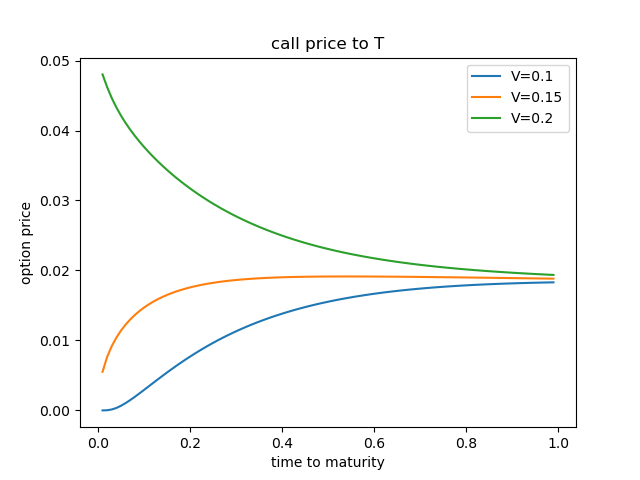
\includegraphics[width=10cm]{./figures/call2T.png}
    \caption{Call option price with regard to time to maturity}\label{call2t}
\end{figure}

\begin{figure}[ht]
    \centering
    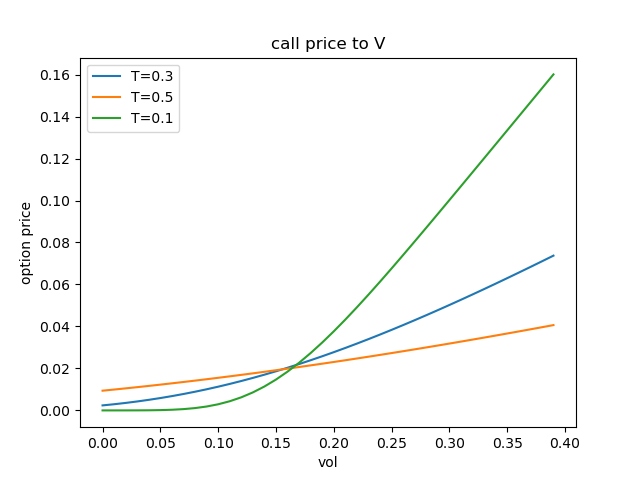
\includegraphics[width=10cm]{./figures/call2V.png}
    \caption{Call option price with regard to volatility}\label{call2v}
\end{figure}

From figure \ref{call2t}, we can find that in contrast to Black-Scholes model, the value of call option price under mean-reverting model is not always increasing as time to maturity increases; From figure \ref{call2v}, by contrast, the call option price does not converge to zero as volatility goes to zero. In addition, \cite{grunbichler_valuing_1996} also shows that $V$ has less influence of the current value of the call option than in Black-Scholes model. For these reasons, we conclude that Black-Scholes model is not an appropriate auxiliary model and in the next section, we discuss that using the square root mean-reverting model as the auxiliary model.

\subsection{Using square root mean-reverting model as auxiliary model}

Recall the mean-reverting CEV model with $\gamma=\frac{1}{2}$

\begin{equation}
    d V_t=\kappa(m - V_t) d t+\sigma \sqrt{V_t} d W_t
\end{equation}

We are going to use it as our auxiliary model as it captures the mean-reverting property of general mean-reverting CEV models. \cite{grunbichler_valuing_1996} gives an explicit solution to this model. Denote the call option price $\bar{w}$ with strike $K$, constant risk-free rate $r$, time to maturity $T$ and no expected premium for volatility risk is paid, its price is given by

\begin{equation}\label{aux call price}
    \begin{aligned}
        \bar{w}=&  e^{ -(\kappa+r) T} V Q(x K ; \nu+4, \lambda) \\
        &+ m e^{-r T}(1-e^{-\kappa T}) Q(xK ; \nu+2, \lambda) \\
        &-e^{-r T} K Q(x K; \nu, \lambda)
        \end{aligned}
\end{equation}

\noindent where

$$
\begin{aligned}
    &x=\frac{4 \kappa}{\sigma^{2}(1-e^{-\kappa T})} \\
    &\nu=\frac{4 \kappa m}{\sigma^{2}}, \\
    &\lambda= e^{-\kappa T}x V
    \end{aligned}
$$

\noindent and $Q(xK ; \nu+i, \lambda)$ is the complementary distribution function for the non-central chi-squared density with $\nu + i$ degrees of freedom and non-centrality parameter $\lambda$.

Define the infinitesimal generators $\bar{\mathcal{L}}$ for square root mean-reverting model and $\mathcal{L}$ for mean-reverting CEV model

\begin{equation}\label{inf gen1}
    \begin{aligned}
        \mathcal{L} w&= \frac{\partial w}{\partial t}+\kappa(m - V) \frac{\partial w}{\partial V}+\frac{1}{2} \sigma^{2} V^{2\gamma} \frac{\partial^{2} w}{\partial V^{2}} \\
        \bar{\mathcal{L}} w &= \frac{\partial w}{\partial t}+\kappa(m - V) \frac{\partial w}{\partial V}+\frac{1}{2} \sigma^{2} V \frac{\partial^{2} w}{\partial V^{2}}
    \end{aligned}
\end{equation}

Subtract infinitesimal generators in equation\eqref{inf gen1}, we get the mis-pricing formula for using square root mean-reverting model

$$
\delta = (\mathcal{L} - \bar{\mathcal{L}}) \bar{w} = \frac{1}{2} \sigma^{2} (V^{2\gamma} - V) \frac{\partial^{2} w}{\partial V^{2}}
$$

\noindent We can then use the approximation formula discussed in \ref{sec: 2.2} to price call options under mean-reverting CEV model\footnote{Put options can be priced easily in the same way}

\begin{equation} \label{cev approx formula}
    w_{N}(t, x)=\bar{w}(t,x)+\sum_{n=0}^{N} \frac{(T-t)^{n+1}}{(n+1) !} \delta_{n}(t, x)
\end{equation}

\noindent where

\begin{equation}\label{mispricing}
    \begin{aligned}
        &\delta_0 = \delta = \frac{1}{2} \sigma^{2} (V^{2\gamma} - V) \frac{\partial^{2} w}{\partial V^{2}} \\
        &\delta_{n}(t, x)=L \delta_{n-1}(t, x)- r\delta_{n-1}(t, x)
        \end{aligned}
\end{equation}

Finally we get a closed form approximating formula for call options under mean-reverting CEV model. But notice that the call price \eqref{aux call price} contains non-square chi square distribution functions, applying infinitesimal generator $\mathcal{L}$ on it can be a hard point and in the next section we are going to talk about how to derive partial derivatives of distribution function $Q(\cdot | \nu+i, \lambda)$.

\subsection{Derivatives of non-central chi-square distribution function}
\label{sec: 3.2}

In this section, methods\footnote{Methods are inspired by \cite{hossain_comparison_2019}, who use to calculate the Greeks of options under CEV model} are given to calculate the derivatives of call option price $\bar{w}$ to time $t$ and volatility index $V$. We have already discussed in \ref{sec: 3.2} the call option prices $\bar{w}$ under square root mean-reverting model, where

\begin{equation}\label{cev param}
    \begin{aligned}
        &x K=\frac{4 \kappa}{\sigma^{2}(1-e^{-\kappa T})} K\\
        &\lambda=x e^{-\kappa T} V = \frac{4 \kappa e^{-\kappa T}}{\sigma^{2}(1-e^{-\kappa T})} V
        \end{aligned}
\end{equation}

Based on equation\eqref{cev param}, we can calculate partial derivatives of $x$ and $\lambda$ with regard to $V$ and $t$

\begin{equation}\label{params dv}
    \begin{gathered}
        \frac{\partial (x K)}{\partial V}=0\\
        \frac{\partial \lambda}{\partial V}=x e^{-\kappa T}  = \frac{4 \kappa e^{-\kappa T}}{\sigma^{2}(1-e^{-\kappa T})}\\
    \end{gathered}
\end{equation}

\begin{equation}\label{params dt}
    \begin{aligned}
        \frac{\partial (x K)}{\partial t}&= \frac{-\kappa e^{-\kappa T}}{1 - e^{-\kappa T}} \cdot  xK\\
        \frac{\partial \lambda}{\partial t}& =\frac{-\kappa e^{-\kappa T}}{1 - e^{-\kappa T}} \cdot  xV
    \end{aligned}
\end{equation}

Besides, using the relationship between the complementary cumulative distribution function(ccdf) $Q(xK; \nu+i, \lambda)$, the cumulative distribution function(cdf) $F(xK; \nu+i, \lambda)$ and the probability density function(pdf) $p(xK; \nu+i, \lambda)$ we can derive

\begin{equation}\label{q dx}
    \begin{aligned}
        \frac{\partial Q(xK; \nu, \lambda)}{\partial x}&=\frac{\partial[1-F(xK; \nu, \lambda)]}{\partial x} \\ 
        &=-\frac{\partial F(xK; \nu, \lambda)]}{\partial x} \\
        &=-p(xK; \nu, \lambda)
        \end{aligned}
\end{equation}

\begin{equation}\label{q dlambda}
    \begin{aligned}
        \frac{\partial Q(xK, \nu, \lambda)}{\partial \lambda}&=\frac{\partial[1-F(xK ; \nu, \lambda)]}{\partial \lambda}\\
        &=-\frac{\partial F(xK ; \nu, \lambda)]}{\partial \lambda} \\
        &=-p(xK ; \nu+2, \lambda)
    \end{aligned}
\end{equation}

Combining equation\eqref{params dt}, \eqref{q dx}, \eqref{q dlambda} to use chain rule we can get partial derivative of $Q(w, \nu, \lambda)$ to time $t$

\begin{equation}\label{q dt}
    \begin{aligned}
        \frac{\partial Q}{\partial t}&= \frac{\partial Q}{\partial (xK)}\frac{\partial (xK)}{\partial t} + \frac{\partial Q}{\partial \lambda} \frac{\partial \lambda}{\partial t} \\
        &= p(xK; \nu, \lambda) \cdot \frac{\kappa e^{-\kappa T}}{1 - e^{-\kappa T}}\cdot xK + p(x ; \nu+2, \lambda) \cdot\frac{\kappa e^{-\kappa T}}{1 - e^{-\kappa T}}\cdot x V \\
        &= \frac{\kappa x e^{-\kappa T}}{1 - e^{-\kappa T}} \left( K p(x, \nu, \lambda)  + V p(x ; \nu+2, \lambda)\right)
    \end{aligned}
\end{equation}

\noindent Similarly combining equation\eqref{params dv}, \eqref{q dx}, \eqref{q dlambda} we can get partial derivative of $Q(w, \nu, \lambda)$ to volatility $V$

\begin{equation}\label{q dv}
    \begin{aligned}
        \frac{\partial Q}{\partial V}&= \frac{\partial Q}{\partial x}\frac{\partial x}{\partial V} + \frac{\partial Q}{\partial \lambda} \frac{\partial \lambda}{\partial V} \\
        &= - x e^{-\kappa T} p(x ; \nu+2, \lambda)
    \end{aligned}
\end{equation}

Thus we can calculate delta of call option

\begin{equation}
    \begin{aligned}
        \Delta_{\bar{w}}&= \frac{\partial \bar{w}}{\partial V} \\
        &= e^{ -(\kappa+r) T} [Q(x K ; \nu+4, \lambda) - xV e^{-\kappa T} p(xK ; \nu+6, \lambda) \\
        &- mx (1-e^{-\kappa T}) p(xK ; \nu+4, \lambda) + xK p(xK ; \nu+2, \lambda)]
        \end{aligned}
\end{equation}

As is seen that pdf in previous equation are all with 2 higher degrees of freedom. However, pdf with higher degrees of freedom require us to re-calculate pdf; Besides, result of approximating pdf with higher degrees of freedom may be inaccurate. To let degrees of freedom $\lambda$ of pdf bounded in some range, we consider the following relationship proposed by \cite{cohen_noncentral_1988}

\begin{equation}\label{h2l}
    p(xK ; \nu+2, \lambda)=\frac{xK}{\lambda} p(xK ; \nu-2, \lambda)-\frac{\nu-2}{\lambda} p(xK ; \nu, \lambda)
\end{equation}

\noindent Using \eqref{h2l} we can rewrite $\Delta_{\bar{w}}$ as

\begin{equation}
    \begin{aligned}
        \Delta_{\bar{w}}&= \frac{\partial \bar{w}}{\partial V} \\
        &= e^{ -(\kappa+r) T} [Q(x K ; \nu+4, \lambda) \\
        &- xV e^{-\kappa T} (\frac{K}{e^{-\kappa T} V} p(xK ; \nu+2, \lambda)-\frac{\nu+2}{\lambda} p(xK ; \nu+4, \lambda) ) \\
        &- mx (1-e^{-\kappa T}) p(xK ; \nu+4, \lambda) + xK p(xK ; \nu+2, \lambda)] \\
        & = e^{ -(\kappa+r) T} [Q(x K ; \nu+4, \lambda) - mx (1-e^{-\kappa T}) p(xK ; \nu+4, \lambda) + (\nu+2 )p(xK ; \nu+4, \lambda)]
        \end{aligned}
\end{equation}

Next we calculate the partial derivatives of pdf $p(x; \nu, \lambda)$ to $V$ and $t$ in order to calculate gamma and apply infinitesimal generator on the mis-pricing formula. \cite{cohen_noncentral_1988} proposes the recurrence relations for $p$, it's also been used in \cite{hossain_comparison_2019} to calculate the Greeks of options under CEV models, which is given by

\begin{equation}\label{pdf1}
    \begin{gathered}
        \frac{\partial p(xK;\nu,\lambda)}{\partial \lambda}=\frac{1}{2}[-p(xK ; v, \lambda)+p(xK ; v+2, \lambda)] \\
        \frac{\partial p(xK;\nu,\lambda)}{\partial (xK)}=\frac{1}{2}[-p(xK ; v, \lambda)+p(xK ; v-2, \lambda)]
    \end{gathered}
\end{equation}

% \noindent It is shown that the partial derivative of pdf $p(x; \nu, \lambda)$ to degrees of freedom $\lambda$ is a combination of original pdf $p(x; \nu, \lambda)$ and 2 degrees higher pdf $p(x; \nu+2, \lambda)$; The partial derivative of pdf $p(x; \nu, \lambda)$ to $x$ is a combination of original pdf $p(x; \nu, \lambda)$ but 2 degrees lower pdf $p(x; \nu+2, \lambda)$. By using the transformation of \eqref{h2l}

% \begin{equation}\label{l2h}
%     p(xK ; \nu-2, \lambda)=\frac{\lambda}{xK} p(xK ; \nu+2, \lambda)+\frac{v-2}{xK} p(xK ; \nu, \lambda)
% \end{equation}

% \noindent We can rewrite \eqref{pdf1} to

\noindent Combining it with equation\eqref{params dv}, \eqref{params dt} gives

\begin{equation}\label{pdf diff}
    \begin{aligned}
        \frac{\partial p}{\partial t}&= \frac{\partial p}{\partial (xK)}\frac{\partial (xK)}{\partial t} + \frac{\partial p}{\partial \lambda} \frac{\partial \lambda}{\partial t} \\
        &= \frac{-\kappa x e^{-\kappa T}}{2(1 - e^{-\kappa T})} \left[Vp(xK ; v+2, \lambda) - (K+V) p(xK ; v, \lambda) + K p(xK ; v-2, \lambda)\right]\\
        \frac{\partial p}{\partial V} &= \frac{\partial p}{\partial (xK)}\frac{\partial (xK)}{\partial V} + \frac{\partial p}{\partial \lambda} \frac{\partial \lambda}{\partial V} \\
        &= \frac{x e^{-\kappa T}}{2} [-p(xK ; v, \lambda)+p(xK ; v+2, \lambda)]
    \end{aligned}
\end{equation}

\noindent Besides, by using the transformation of \eqref{h2l}

\begin{equation}\label{l2h}
    p(xK ; \nu-2, \lambda)=\frac{\lambda}{xK} p(xK ; \nu+2, \lambda)+\frac{v-2}{xK} p(xK ; \nu, \lambda)
\end{equation}

\noindent $p(xK;\nu-2,\lambda)$ in \eqref{pdf diff} can be substituted by

\begin{equation}\label{pdf2}
    \begin{aligned}
        \frac{\partial p(xK;\nu,\lambda)}{\partial (xK)}&=\frac{1}{2}[-p(xK ; v, \lambda)+p(xK ; v-2, \lambda)]\\
        &=\frac{1}{2}\left[(\frac{v-2}{xK}-1) p(xK ; \nu, \lambda) + \frac{\lambda}{xK} p(xK ; \nu+2, \lambda))\right]
    \end{aligned}
\end{equation}

Thus gamma of call option under square root mean-reverting model is then

\begin{equation}\label{gamma}
    \begin{aligned}
        \begin{aligned}
            \Gamma_{\bar{w}}&= \frac{\partial \Delta_{\bar{w}}}{\partial V} \\
            &= \frac{xe^{-(2\kappa +r )T}}{2} [mx(1-e^{-\kappa T})(p(xK ; \nu+4, \lambda)-p(xK+6 ; \nu, \lambda)) \\
            &+ \nu p(xK+6 ; \nu, \lambda) - (\nu+2)p(xK+4 ; \nu, \lambda)]
            \end{aligned}
    \end{aligned}
\end{equation}

From \eqref{mispricing} we know that $\delta = \frac{1}{2} \sigma^2 (V^{2\gamma}-V) \Gamma_{\bar{w}}$, all terms have been solved from above. In essence, during expansion, we can solve partial derivatives of cdf $Q(xK;\nu,\lambda)$ and pdf $p(xK;\nu,\lambda)$ explicitly. And for those pdf with degrees out of bounds, we use \eqref{l2h} and \eqref{h2l} to adjust them, making degrees of freedom within our desired range. Finally we can get a closed-form approximation formula for all mean-reverting CEV model. The expansions in approximating formula can be computed once for all, we can solve it manually or use symbolic language.

\section{Approximating options under double Heston model}

\cite{gatheral_consistent_nodate} proposes volatility with double mean-reverting dynamics

$$
    \begin{aligned}
        d V_t &=-\kappa\left(V_t-V^{\prime}(t)\right) d t+\eta_{1} V^{\prime \alpha}_t  d W_1(t) \\
        d V^{\prime}_t &=-c\left(V^{\prime}_t-m\right) d t+\eta_{2} V^{\prime \beta}_t d W_{2}(t)
    \end{aligned}
$$

\noindent where $\alpha, \beta \in [\frac{1}{2},1]$.

\begin{itemize}
    \item It's called Double Heston model in the case $\alpha=\beta=\frac{1}{2}$.
    \item The case $\alpha=\beta=1$ Double Log-normal model.
    \item And the general Double CEV model.
\end{itemize}

From our previous work we can price options with $V_t$ following heston dynamics and $V^{\prime}$ following any mean-reverting CEV process, the model is thus

\begin{equation}\label{heston cev}
    \begin{aligned}
        d V_t &=-\kappa\left(V_t-V^{\prime}(t)\right) d t+\eta_{1} \sqrt{V_t} d W_1(t) \\
        d V^{\prime}_t &=-c\left(V^{\prime}_t-m\right) d t+\eta_{2} V^{\prime \beta}_t d W_{2}(t)
    \end{aligned}
\end{equation}

Define infinitesimal generator $\mathcal{L}$ for \eqref{heston cev} and we still use square root mean-reverting model as our auxiliary model

\begin{equation}\label{inf gen2}
    \begin{aligned}
        \mathcal{L} w&= \frac{\partial w}{\partial t}+\kappa(V^{\prime} - V) \frac{\partial w}{\partial V}+\frac{1}{2} \eta_1^{2} V \frac{\partial^{2} w}{\partial V^{2}} \\
        &+ \frac{\partial w}{\partial t}+c(m^{\prime} - V^{\prime}) \frac{\partial w}{V^{\prime}}+\frac{1}{2} \eta_2^{2} V \frac{\partial^{2} w}{V^{\prime 2}}\\
        \bar{\mathcal{L}} w &= \frac{\partial w}{\partial t}+\kappa(m - V) \frac{\partial w}{\partial V}+\frac{1}{2} \eta_1 V \frac{\partial^{2} w}{\partial V^{2}}
    \end{aligned}
\end{equation}

\noindent Mis-pricing formula for it is then

$$
\begin{aligned}
    \delta = (\mathcal{L} - \bar{\mathcal{L}}) \bar{w} &= \kappa(V^{\prime}-m)\frac{\partial w}{\partial V} \\
    &= \kappa(V^{\prime}-m) \Gamma_{\bar{w}}
\end{aligned}
$$

\noindent where $\Gamma_{\bar{w}}$ is given in \eqref{gamma}.
% \chapter{Case Study}
% All information about formatting a dissertation can be found on the library website at www.stevens.edu/library/services/phd.html.  Formatting information gets updated occasionally, so it is always good to check the requirements before submitting your dissertation.  

% It is not required, but is strongly suggested that you make an appointment at the library to have the format of your dissertation reviewed before the final submission.  Dissertations can be rejected if they do not adhear to the formatting requirements.   

% All information about formatting a dissertation can be found on the library website at www.stevens.edu/library/services/phd.html.  Formatting information gets updated occasionally, so it is always good to check the requirements before submitting your dissertation.  
% It is not required, but is strongly suggested that you make an appointment at the library to have the format of your dissertation reviewed before the final submission.  Dissertations can be rejected if they do not adhear to the formatting requirements.   
% All information about formatting a dissertation can be found on the library website at www.stevens.edu/library/services/phd.html.  Formatting information gets updated occasionally, so it is always good to check the requirements before submitting your dissertation.  

% \begin{table}[htp]

% \begin{center}
% \begin{tabular}{|l|c|p{3.0in}|}
% \hline
% \multicolumn{3}{|c|}{Theoretical Dissertation Timeline}\\ \hline
% Taskt&Time to Finish&Notes\\ \hline
% Problem statement&10 hours&Initially very upbeat.\\ \hline
% Research&3 days&Literature search to very previous studies.\\ \hline
% Reformulation&4 hours&Presented and accepted by advisor\\ \hline
% Research&20 days&Literature search to very previous  studies.\\ \hline
% Experiments&14 days&Do some experiments and get results.\\ \hline
% Format&1 day&Understand format guidelines for paper.\\ \hline
% Write&years&Write the paper.\\ \hline
% Revise&not too long&Proof read, etc.\\ \hline
% Format&1-3 days&Verify correct report format is used.\\ \hline
% See Library&1 hour&Meet with Doris to verify formatting.\\ \hline
% Defend&1 day&Defend your research.\\ \hline
% Revise&0 hours&It was perfect the first time.\\ \hline
% Submit&1 day&Submit final dissertation to the library.\\ \hline
% \end{tabular}
% \end{center} 

% \caption{Table of Tasks}\label{tab:erptsqfit}
% \end{table}
% It is not required, but is strongly suggested that you make an appointment at the library to have the format of your dissertation reviewed before the final submission.  Dissertations can be rejected if they do not adhear to the formatting requirements.   
% All information about formatting a dissertation can be found on the library website at www.stevens.edu/library/services/phd.html.  Formatting information gets updated occasionally, so it is always good to check the requirements before submitting your dissertation.  
% It is not required, but is strongly suggested that you make an appointment at the library to have the format of your dissertation reviewed before the final submission.  Dissertations can be rejected if they do not adhear to the formatting requirements.   
% All information about formatting a dissertation can be found on the library website at www.stevens.edu/library/services/phd.html.  Formatting information gets updated occasionally, so it is always good to check the requirements before submitting your dissertation.  

% It is not required, but is strongly suggested that you make an appointment at the library to have the format of your dissertation reviewed before the final submission.  Dissertations can be rejected if they do not adhear to the formatting requirements.   



% \section{Further Analysis}  

% \subsection*\normalsize\emph{Paper}
% The original copy of the dissertation must be produced on good quality 8 1/2$''$ x 11$''$, 20 pound acid-free white paper. The paper should not be stapled, punched, bound, colored or printed on letterhead.

% The two additional copies of the dissertation can be photocopied or produced on copier or laser paper.

% \subsection*\normalsize\emph{Ink}
% Black ink only is used to print your report.  If a graph or photograph contains color, that is fine. 

% Latex is used to help in the printing of formulas.   The following formula would be difficult to reproduce in Microsoft Word: 
%  \[
%         \frac{d}{dx}\left( \int_{0}^{x} f(u)\,du\right)=f(x).
%      \]

% This Report was produced by LaTeX\footnote {\LaTeX\ is a fun typesetting program. Single space is used in footnotes.} written by Barbara Arnett.  Barbara is not an expert with LaTeX, and anyone using LaTeX does not need to use this template.  It is simply provided to help with formatting, specifically with page numbers and images.  


% %this subsection heading below will not show up in the table of contents.
% \subsection*\normalsize\emph{Graphics} 

% Graph paper may be used for original drawings, charts or illustrations. Original drawings may be in color or black and white, however, color is allowed for illustrations only; all text must appear in black. The original thesis must contain the original graphic or illustration, not a photocopy of the drawing, graphic or illustration.

% If formulas and diagrams contain subscript and superscript characters, ensure they are large enough to read when printed in the final paper. 

% \begin{figure}[htp]
% \centering
% 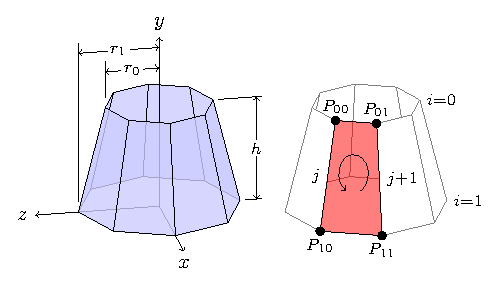
\includegraphics{3d-cone.pdf}
% \caption{3D Cone}\label{fig:3d-cone}
% \end{figure}

% Photographs
% Glossy prints of good reproducible quality, either black or white or color may be used. Photographs can be printed on 8 1/2$''$ x 11$''$ glossy finish paper, however, margin and page number requirements as stated above still apply for pages containing photographs. When attaching photographs to paper, double-sided tape may be used which causes the least amount of damage to the original paper. 

% Graphics that are oriented in a landscape position must be done in a manner that retains the page numbering in the upper right hand corner, as shown in figure 3.2.  This can be difficult in Microsoft Word, but it is possible.  To do this in Microsoft Word, create a new section, change the page to landscape, and place the page number in a text box.  The text box then is rotated on the landscape page.    Then begin a new section and resume portrait orientation.

% \begin{sidewaysfigure}
% \centering
% 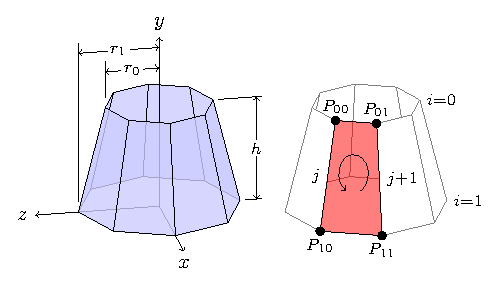
\includegraphics[height=5.0in, width=7.5in]{3d-cone.pdf}
% \caption{This is an example of a landscape image within a page.  Note that the page number remains in the upper right hand corner of the page when the page is in the portrait position.}
% \end{sidewaysfigure}




% \chapter{Recommendations}

% Glossy prints of good reproducible quality, either black or white or color may be used. Photographs can be printed on 8$''$ x 11$''$ glossy finish paper, however, margin and page number requirements as stated above still apply for pages containing photographs. When attaching photographs to paper, double-sided tape may be used which causes the least amount of damage to the original paper.

% The format of footnotes and the bibliography are to be prepared in accordance with standard practice in the field in which one is working. Documentation formatting style must be discussed with and accepted by the advisor. See further information on Reference Styles below.

% The suggested typeface for dissertations is 10 to 12 point Arial. Other suggested fonts are Times New Roman and Helvetica. Script and italic fonts should not be used except as needed in the body of the paper. Consistency should be maintained throughout the paper, using the same font for all text, diagrams, etc. on all pages.

% Electronic material, such as CDs and multimedia can accompany the dissertation. Each copy should be accompanied with a labeled CD. When bound, these are placed in an envelope in the back of the dissertation.  Oversized materials (pages greater than 8 1/2$''$ x 11$''$) can be included in the paper if necessary. Oversized pages should be folded so that 1$''$ on the left hand binding edge remains, allowing the page to be opened once the paper is bound.

% The reference style used for formatting the paper must be confirmed with your department and advisor. Frequently used styles are the APA (American Psychological Association), MLA (Modern Language Association) and AMA (American Medical Association) styles. Style guides and manuals are available for each style. Page headers are not to be used.


% \section{The Focus Group}    

% Glossy prints of good reproducible quality, either black or white or color may be used. Photographs can be printed on 8 1/2$''$ x 11$''$ glossy finish paper, however, margin and page number requirements as stated above still apply for pages containing photographs. When attaching photographs to paper, double-sided tape may be used which causes the least amount of damage to the original paper.

% The format of footnotes and the bibliography are to be prepared in accordance with standard practice in the field in which one is working. Documentation formatting style must be discussed with and accepted by the advisor. See further information on Reference Styles below.
% \subsection{focusing}

% The suggested typeface for dissertations is 10 to 12 point Arial. Other suggested fonts are Times New Roman and Helvetica. Script and italic fonts should not be used except as needed in the body of the paper. Consistency should be maintained throughout the paper, using the same font for all text, diagrams, etc. on all pages.

% \begin{table}[htp]

% \begin{center}
% \begin{tabular}{|l|c|p{3.0in}|}
% \hline
% \multicolumn{2}{|c|}{Another Timeline}\\ \hline
% Taskt&Notes\\ \hline
% Problem statement&Initially very upbeat.\\ \hline
% Research&Literature search to very previous studies.\\ \hline
% Reformulation&Presented and accepted by advisor\\ \hline
% Research&Literature search to very previous  studies.\\ \hline
% Experiments&Do some experiments and get results.\\ \hline
% Format&Understand format guidelines for paper.\\ \hline
% Write&Write the paper.\\ \hline
% Revise&Proof read, etc.\\ \hline
% Format&Verify correct report format is used.\\ \hline
% See Library&Meet with Doris to verify formatting.\\ \hline
% Defend&Defend your research.\\ \hline
% Revise&It was perfect the first time.\\ \hline
% Submit&Submit final dissertation to the library.\\ \hline
% \end{tabular}
% \end{center} 
% \caption{Timeline 2}\label{tab:erptsqfit2}
% \end{table}

% Electronic material, such as CDs and multimedia can accompany the dissertation. Each copy should be accompanied with a labeled CD. When bound, these are placed in an envelope in the back of the dissertation.  Oversized materials (pages greater than 8 1/2$''$ x 11$''$) can be included in the paper if necessary. Oversized pages should be folded so that 1½" on the left hand binding edge remains, allowing the page to be opened once the paper is bound.

% The reference style used for formatting the paper must be confirmed with your department and advisor. Frequently used styles are the APA (American Psychological Association), MLA (Modern Language Association) and AMA (American Medical Association) styles. Style guides and manuals are available for each style. Page headers are not to be used.

% \chapter{Summary and Conclusion}

% Glossy prints of good reproducible quality, either black or white or color may be used. Photographs can be printed on 8 1/2$''$ x 11$''$ glossy finish paper, however, margin and page number requirements as stated above still apply for pages containing photographs. When attaching photographs to paper, double-sided tape may be used which causes the least amount of damage to the original paper.

% The format of footnotes and the bibliography are to be prepared in accordance with standard practice in the field in which one is working. Documentation formatting style must be discussed with and accepted by the advisor. See further information on Reference Styles below.

% The suggested typeface \cite{henderson_intellectual_2009} for dissertations is 10 to 12 point Arial. Other suggested fonts are Times New Roman and Helvetica. Script and italic fonts should not be used except as needed in the body of the paper. Consistency should be maintained throughout the paper, using the same font for all text, diagrams, etc. on all pages.

% Electronic material, such as CDs and multimedia can accompany the dissertation. Each copy should be accompanied with a labeled CD. When bound, these are placed in an envelope in the back of the dissertation.  Oversized materials (pages greater than 8 1/2$''$ x 11$''$) can be included in the paper if necessary. Oversized pages should be folded so that 1½" on the left hand binding edge remains, allowing the page to be opened once the paper is bound.

% The reference style used for formatting the paper must be confirmed with your department and advisor. Frequently used styles are the APA (American Psychological Association), MLA (Modern Language Association) and AMA (American Medical Association) styles. Style guides and manuals are available for each style. Page headers are not to be used.

\begin{appendix}
\chapter{Appendix A Mean-reverting CEV model results}
\label{mrcev}

\begin{table}[ht]
  \centering
  \caption{Mean-reverting CEV Results 1}
  \begin{tabular}{rrrrrr}
  \toprule
    vol &       benchmark &       N=0 &       N=1 &       N=2 &       N=3 \\
  \midrule
  0.100 & 0.001765 & 0.002282 & 0.001963 & 0.001814 & 0.001771 \\
  0.125 & 0.005116 & 0.005492 & 0.005304 & 0.005185 & 0.005144 \\
  0.150 & 0.011722 & 0.011733 & 0.011769 & 0.011757 & 0.011742 \\
  0.175 & 0.022066 & 0.021711 & 0.021911 & 0.022003 & 0.022020 \\
  0.200 & 0.035341 & 0.035023 & 0.035223 & 0.035335 & 0.035367 \\
  0.225 & 0.050630 & 0.050438 & 0.050546 & 0.050612 & 0.050640 \\
  0.250 & 0.066827 & 0.066771 & 0.066807 & 0.066831 & 0.066844 \\
  0.275 & 0.083368 & 0.083381 & 0.083389 & 0.083394 & 0.083398 \\
  0.300 & 0.100014 & 0.100047 & 0.100048 & 0.100049 & 0.100050 \\
  0.325 & 0.116674 & 0.116721 & 0.116721 & 0.116721 & 0.116721 \\
  0.350 & 0.133341 & 0.133395 & 0.133395 & 0.133395 & 0.133395 \\
  0.375 & 0.150010 & 0.150070 & 0.150070 & 0.150070 & 0.150070 \\
  0.400 & 0.166680 & 0.166744 & 0.166744 & 0.166744 & 0.166744 \\
  \bottomrule
  \end{tabular}
  \small{$T=0.1,K=0.15, \kappa =  4,m=0.15, \sigma =0.15, \gamma = 0.15$}
  \end{table}

\begin{table}[ht]
\centering
\caption{Mean-reverting CEV Results 2}
\begin{tabular}{rrrrrr}
\toprule
  vol &       benchmark &       N=0 &       N=1 &       N=2 &       N=3 \\
\midrule
0.100 & 0.008524 & 0.009945 & 0.009626 & 0.009228 & 0.008914 \\
0.125 & 0.011446 & 0.012059 & 0.011926 & 0.011763 & 0.011629 \\
0.150 & 0.014988 & 0.014888 & 0.014913 & 0.014949 & 0.014971 \\
0.175 & 0.019049 & 0.018438 & 0.018590 & 0.018788 & 0.018938 \\
0.200 & 0.023748 & 0.022704 & 0.022945 & 0.023257 & 0.023502 \\
0.225 & 0.028813 & 0.027653 & 0.027940 & 0.028316 & 0.028615 \\
0.250 & 0.034477 & 0.033220 & 0.033515 & 0.033902 & 0.034216 \\
0.275 & 0.040438 & 0.039316 & 0.039585 & 0.039942 & 0.040238 \\
0.300 & 0.046773 & 0.045836 & 0.046061 & 0.046360 & 0.046613 \\
0.325 & 0.053424 & 0.052678 & 0.052850 & 0.053079 & 0.053279 \\
0.350 & 0.060253 & 0.059747 & 0.059867 & 0.060029 & 0.060175 \\
0.375 & 0.067260 & 0.066965 & 0.067043 & 0.067149 & 0.067248 \\
0.400 & 0.074406 & 0.074276 & 0.074323 & 0.074386 & 0.074448 \\
\bottomrule
\end{tabular}
\small{$T=0.3,K=0.15, \kappa = 4,m=0.15, \sigma = 0.15, \gamma = 0.15$}
\end{table}

\begin{table}[ht]
  \centering
  \caption{Mean-reverting CEV Results 3}
  \begin{tabular}{rrrrrr}
  \toprule
    vol &       benchmark &       N=0 &       N=1 &       N=2 &       N=3 \\
  \midrule
  0.100 & 0.011161 & 0.010017 & 0.010319 & 0.010707 & 0.010977 \\
  0.125 & 0.014896 & 0.014296 & 0.014483 & 0.014653 & 0.014746 \\
  0.150 & 0.019031 & 0.019025 & 0.019081 & 0.019065 & 0.019015 \\
  0.175 & 0.023634 & 0.024130 & 0.024056 & 0.023887 & 0.023722 \\
  0.200 & 0.028525 & 0.029551 & 0.029356 & 0.029063 & 0.028811 \\
  0.225 & 0.033780 & 0.035240 & 0.034937 & 0.034547 & 0.034230 \\
  0.250 & 0.039312 & 0.041156 & 0.040759 & 0.040296 & 0.039931 \\
  0.275 & 0.045297 & 0.047265 & 0.046792 & 0.046272 & 0.045876 \\
  0.300 & 0.051352 & 0.053541 & 0.053004 & 0.052446 & 0.052030 \\
  0.325 & 0.057697 & 0.059959 & 0.059373 & 0.058788 & 0.058362 \\
  0.350 & 0.064114 & 0.066500 & 0.065876 & 0.065276 & 0.064848 \\
  0.375 & 0.070721 & 0.073147 & 0.072496 & 0.071890 & 0.071465 \\
  0.400 & 0.077345 & 0.079886 & 0.079218 & 0.078612 & 0.078196 \\
  \bottomrule
  \end{tabular}
  \small{$T=0.3,K=0.15, \kappa = 4,m=0.15, \gamma = 0.6, \sigma = 0.75$}
\end{table}     

\begin{table}[ht]
  \centering
  \caption{Mean-reverting CEV Results 4}
  \begin{tabular}{rrrrrr}
  \toprule
    vol &       benchmark &       N=0 &       N=1 &       N=2 &       N=3 \\
  \midrule
  0.100 & 0.012213 & 0.014045 & 0.013888 & 0.013574 & 0.013202 \\
  0.125 & 0.013757 & 0.014490 & 0.014421 & 0.014289 & 0.014140 \\
  0.150 & 0.015424 & 0.015298 & 0.015301 & 0.015316 & 0.015346 \\
  0.175 & 0.017197 & 0.016390 & 0.016455 & 0.016592 & 0.016766 \\
  0.200 & 0.019004 & 0.017726 & 0.017842 & 0.018079 & 0.018372 \\
  0.225 & 0.020967 & 0.019282 & 0.019439 & 0.019757 & 0.020145 \\
  0.250 & 0.022990 & 0.021040 & 0.021230 & 0.021610 & 0.022070 \\
  0.275 & 0.025099 & 0.022987 & 0.023200 & 0.023625 & 0.024136 \\
  0.300 & 0.027349 & 0.025111 & 0.025338 & 0.025790 & 0.026332 \\
  0.325 & 0.029779 & 0.027399 & 0.027632 & 0.028095 & 0.028650 \\
  0.350 & 0.032255 & 0.029839 & 0.030071 & 0.030529 & 0.031079 \\
  0.375 & 0.034676 & 0.032417 & 0.032640 & 0.033081 & 0.033612 \\
  0.400 & 0.037324 & 0.035118 & 0.035328 & 0.035742 & 0.036241 \\
  \bottomrule
  \end{tabular}
  \small{$T=0.5,K=0.15, \kappa = 4,m=0.15, \sigma = 0.15, \gamma = 0.15$}
\end{table}

\begin{table}[ht]
  \centering
  \caption{Mean-reverting CEV Results 5}
  \begin{tabular}{rrrrrr}
  \toprule
    vol &       benchmark &       N=0 &       N=1 &       N=2 &       N=3 \\
  \midrule
  0.100 & 0.015724 & 0.014125 & 0.014276 & 0.014597 & 0.014972 \\
  0.125 & 0.017575 & 0.016839 & 0.016938 & 0.017101 & 0.017269 \\
  0.150 & 0.019692 & 0.019535 & 0.019579 & 0.019612 & 0.019614 \\
  0.175 & 0.021633 & 0.022231 & 0.022218 & 0.022139 & 0.022006 \\
  0.200 & 0.023916 & 0.024936 & 0.024865 & 0.024688 & 0.024442 \\
  0.225 & 0.025893 & 0.027654 & 0.027526 & 0.027261 & 0.026920 \\
  0.250 & 0.028110 & 0.030388 & 0.030205 & 0.029860 & 0.029438 \\
  0.275 & 0.030481 & 0.033139 & 0.032903 & 0.032486 & 0.031993 \\
  0.300 & 0.032885 & 0.035909 & 0.035621 & 0.035139 & 0.034585 \\
  0.325 & 0.035172 & 0.038698 & 0.038361 & 0.037818 & 0.037211 \\
  0.350 & 0.037742 & 0.041505 & 0.041120 & 0.040523 & 0.039868 \\
  0.375 & 0.040364 & 0.044329 & 0.043901 & 0.043253 & 0.042557 \\
  0.400 & 0.042932 & 0.047172 & 0.046701 & 0.046006 & 0.045275 \\
  \bottomrule
  \end{tabular}
  \small{$T=0.5,K=0.15, \kappa = 4,m=0.15, \sigma = 0.6, \gamma = 0.75$}
\end{table}

\begin{table}[ht]
  \centering
  \caption{Mean-reverting CEV Results 1 with another nuisance parameter}
  \begin{tabular}{rrrrrr}
  \toprule
    vol &       benchmark &       N=0 &       N=1 &       N=2 &       N=3 \\
  \midrule
  0.100 & 0.012224 & 0.011962 & 0.012092 & 0.012191 & 0.012249 \\
  0.125 & 0.013753 & 0.013575 & 0.013641 & 0.013696 & 0.013741 \\
  0.150 & 0.015348 & 0.015298 & 0.015301 & 0.015316 & 0.015346 \\
  0.175 & 0.017127 & 0.017129 & 0.017073 & 0.017050 & 0.017063 \\
  0.200 & 0.018948 & 0.019067 & 0.018955 & 0.018896 & 0.018893 \\
  0.225 & 0.020895 & 0.021109 & 0.020944 & 0.020852 & 0.020833 \\
  0.250 & 0.023076 & 0.023250 & 0.023037 & 0.022915 & 0.022882 \\
  0.275 & 0.025132 & 0.025487 & 0.025232 & 0.025082 & 0.025037 \\
  0.300 & 0.027426 & 0.027814 & 0.027523 & 0.027350 & 0.027292 \\
  0.325 & 0.029751 & 0.030228 & 0.029905 & 0.029713 & 0.029645 \\
  0.350 & 0.032177 & 0.032724 & 0.032375 & 0.032166 & 0.032091 \\
  0.375 & 0.034672 & 0.035295 & 0.034927 & 0.034705 & 0.034623 \\
  0.400 & 0.037282 & 0.037937 & 0.037555 & 0.037324 & 0.037238 \\
  \bottomrule
  \end{tabular}
  \small{$T=0.5,K=0.15, kappa = 4,m=0.15, \sigma = 0.15, \gamma = 0.15$}
\end{table}

\begin{table}[ht]
  \centering
  \caption{Mean-reverting CEV Results 2 with another nuisance parameter}
  \begin{tabular}{rrrrrr}
  \toprule
    vol &       benchmark &       N=0 &       N=1 &       N=2 &       N=3 \\
  \midrule
  0.100 & 0.015666 & 0.015823 & 0.015735 & 0.015693 & 0.015682 \\
  0.125 & 0.017610 & 0.017630 & 0.017612 & 0.017609 & 0.017606 \\
  0.150 & 0.019588 & 0.019535 & 0.019579 & 0.019612 & 0.019614 \\
  0.175 & 0.021602 & 0.021532 & 0.021632 & 0.021695 & 0.021702 \\
  0.200 & 0.023603 & 0.023615 & 0.023765 & 0.023854 & 0.023863 \\
  0.225 & 0.025964 & 0.025780 & 0.025974 & 0.026083 & 0.026094 \\
  0.250 & 0.028169 & 0.028020 & 0.028254 & 0.028377 & 0.028389 \\
  0.275 & 0.030495 & 0.030332 & 0.030600 & 0.030734 & 0.030746 \\
  0.300 & 0.032966 & 0.032711 & 0.033008 & 0.033149 & 0.033161 \\
  0.325 & 0.035109 & 0.035152 & 0.035475 & 0.035619 & 0.035629 \\
  0.350 & 0.037603 & 0.037652 & 0.037995 & 0.038139 & 0.038149 \\
  0.375 & 0.040286 & 0.040205 & 0.040565 & 0.040708 & 0.040716 \\
  0.400 & 0.042783 & 0.042810 & 0.043182 & 0.043322 & 0.043329 \\
  \bottomrule
  \end{tabular}
  \small{$T=0.5,K=0.15, \kappa = 4,m=0.15, \sigma = 0.6, \gamma = 0.75$}
\end{table}




\chapter{Appendix B Heston plus CEV model Results}

\begin{table}[ht]
  \centering
  \caption{Heston plus CEV Results 1}
  \begin{tabular}{rrrrrr}
  \toprule
    vol &       Benchmark &       N=0 &       N=1 &       N=2 &       N=3 \\
  \midrule
  0.100 & 0.041967 & 0.039631 & 0.039755 & 0.040114 & 0.040610 \\
  0.125 & 0.044725 & 0.042462 & 0.042589 & 0.042928 & 0.043388 \\
  0.150 & 0.047219 & 0.045343 & 0.045469 & 0.045788 & 0.046212 \\
  0.175 & 0.050433 & 0.048268 & 0.048392 & 0.048690 & 0.049081 \\
  0.200 & 0.053086 & 0.051234 & 0.051354 & 0.051632 & 0.051991 \\
  0.225 & 0.055863 & 0.054236 & 0.054351 & 0.054609 & 0.054938 \\
  0.250 & 0.058803 & 0.057272 & 0.057381 & 0.057620 & 0.057920 \\
  0.275 & 0.061546 & 0.060337 & 0.060440 & 0.060660 & 0.060933 \\
  0.300 & 0.064546 & 0.063429 & 0.063526 & 0.063728 & 0.063976 \\
  0.325 & 0.067506 & 0.066545 & 0.066635 & 0.066820 & 0.067045 \\
  0.350 & 0.070821 & 0.069683 & 0.069766 & 0.069935 & 0.070139 \\
  0.375 & 0.073777 & 0.072840 & 0.072917 & 0.073070 & 0.073254 \\
  0.400 & 0.076874 & 0.076014 & 0.076085 & 0.076224 & 0.076390 \\
  \bottomrule
  \end{tabular}
  \small{$\rho = 0.5,T=0.5,K=0.15, \kappa_1 =4, \kappa_2 =2, \theta =0.2, \sigma_1 = 0.3, \sigma_2 =0.8, \gamma = 1.6$}
\end{table}

\begin{table}[ht]
  \centering
  \caption{Heston plus CEV Results 2}
  \begin{tabular}{rrrrrr}
  \toprule
    vol &       Benchmark &       N=0 &       N=1 &       N=2 &       N=3 \\
  \midrule
  0.100 & 0.028731 & 0.026700 & 0.027060 & 0.027694 & 0.028228 \\
  0.125 & 0.034194 & 0.032408 & 0.032747 & 0.033302 & 0.033765 \\
  0.150 & 0.040194 & 0.038481 & 0.038788 & 0.039262 & 0.039654 \\
  0.175 & 0.046324 & 0.044856 & 0.045125 & 0.045522 & 0.045847 \\
  0.200 & 0.052647 & 0.051476 & 0.051705 & 0.052030 & 0.052296 \\
  0.225 & 0.059171 & 0.058291 & 0.058481 & 0.058743 & 0.058956 \\
  0.250 & 0.065856 & 0.065258 & 0.065413 & 0.065621 & 0.065789 \\
  0.275 & 0.072707 & 0.072344 & 0.072467 & 0.072629 & 0.072760 \\
  0.300 & 0.079774 & 0.079519 & 0.079615 & 0.079740 & 0.079840 \\
  0.325 & 0.086861 & 0.086761 & 0.086835 & 0.086929 & 0.087006 \\
  0.350 & 0.094048 & 0.094052 & 0.094109 & 0.094180 & 0.094237 \\
  0.375 & 0.101330 & 0.101381 & 0.101423 & 0.101476 & 0.101518 \\
  0.400 & 0.108511 & 0.108736 & 0.108767 & 0.108805 & 0.108837 \\
  \bottomrule
  \end{tabular}
  \small{$rho = 0.5,T=0.3,K=0.15, \kappa = 4, \kappa_2 =2, \theta =0.2, \sigma_1 =0.3, \sigma_2 = 0.8, \gamma = 1.6$}
\end{table}

\begin{table}[ht]
  \centering
  \caption{Heston plus CEV Results 3}
  \begin{tabular}{rrrrrr}
  \toprule
    vol &       Benchmark &       N=0 &       N=1 &       N=2 &       N=3 \\
  \midrule
  0.100 & 0.005247 & 0.004694 & 0.005024 & 0.005205 & 0.005244 \\
  0.125 & 0.012043 & 0.011530 & 0.011918 & 0.012127 & 0.012177 \\
  0.150 & 0.022560 & 0.022034 & 0.022365 & 0.022539 & 0.022587 \\
  0.175 & 0.035793 & 0.035431 & 0.035647 & 0.035760 & 0.035796 \\
  0.200 & 0.050773 & 0.050618 & 0.050732 & 0.050791 & 0.050813 \\
  0.225 & 0.067072 & 0.066709 & 0.066759 & 0.066785 & 0.066795 \\
  0.250 & 0.083152 & 0.083183 & 0.083201 & 0.083211 & 0.083215 \\
  0.275 & 0.099635 & 0.099796 & 0.099802 & 0.099805 & 0.099807 \\
  0.300 & 0.116672 & 0.116454 & 0.116455 & 0.116456 & 0.116457 \\
  0.325 & 0.132955 & 0.133124 & 0.133124 & 0.133125 & 0.133125 \\
  0.350 & 0.149813 & 0.149797 & 0.149797 & 0.149798 & 0.149798 \\
  0.375 & 0.166078 & 0.166472 & 0.166472 & 0.166472 & 0.166472 \\
  0.400 & 0.183073 & 0.183146 & 0.183146 & 0.183146 & 0.183146 \\
  \bottomrule
  \end{tabular}
  \small{$\rho = 0.5,T=0.1,K=0.15, \kappa = 4, \kappa_2 =2, \theta =0.2, \sigma_1 =0.3, \sigma_2 = 0.8, \gamma = 1.6$}
  \end{table}


\begin{table}[ht]
  \centering
  \caption{Heston plus CEV Results 4}
  \begin{tabular}{rrrrrr}
  \toprule
    vol &       Benchmark &       N=0 &       N=1 &       N=2 &       N=3 \\
  \midrule
  0.100 & 0.039308 & 0.039631 & 0.039507 & 0.039361 & 0.039257 \\
  0.125 & 0.042042 & 0.042462 & 0.042336 & 0.042191 & 0.042089 \\
  0.150 & 0.044895 & 0.045343 & 0.045217 & 0.045074 & 0.044975 \\
  0.175 & 0.047644 & 0.048268 & 0.048145 & 0.048005 & 0.047909 \\
  0.200 & 0.050756 & 0.051234 & 0.051114 & 0.050979 & 0.050887 \\
  0.225 & 0.053812 & 0.054236 & 0.054122 & 0.053992 & 0.053904 \\
  0.250 & 0.056708 & 0.057272 & 0.057163 & 0.057039 & 0.056956 \\
  0.275 & 0.060041 & 0.060337 & 0.060234 & 0.060117 & 0.060038 \\
  0.300 & 0.062654 & 0.063429 & 0.063333 & 0.063223 & 0.063148 \\
  0.325 & 0.065996 & 0.066545 & 0.066456 & 0.066352 & 0.066282 \\
  0.350 & 0.069234 & 0.069683 & 0.069600 & 0.069504 & 0.069438 \\
  0.375 & 0.072593 & 0.072840 & 0.072763 & 0.072674 & 0.072613 \\
  0.400 & 0.075404 & 0.076014 & 0.075944 & 0.075861 & 0.075805 \\
  \bottomrule
  \end{tabular}
  \small{$rho = -0.5,T=0.5,K=0.15, \kappa = 4, \kappa_2 =2, \theta =0.2, \sigma_1 =0.3, \sigma_2 = 0.8, \gamma = 1.6$}
  \end{table}

\begin{table}[ht]
  \centering
  \caption{Heston plus CEV Results 5}
  \begin{tabular}{rrrrrr}
  \toprule
    vol &       Benchmark &       N=0 &       N=1 &       N=2 &       N=3 \\
  \midrule
  0.100 & 0.026109 & 0.026700 & 0.026340 & 0.026073 & 0.025953 \\
  0.125 & 0.031726 & 0.032408 & 0.032068 & 0.031820 & 0.031709 \\
  0.150 & 0.038037 & 0.038481 & 0.038173 & 0.037949 & 0.037849 \\
  0.175 & 0.044516 & 0.044856 & 0.044587 & 0.044389 & 0.044302 \\
  0.200 & 0.051039 & 0.051476 & 0.051247 & 0.051077 & 0.051003 \\
  0.225 & 0.058111 & 0.058291 & 0.058101 & 0.057958 & 0.057897 \\
  0.250 & 0.064906 & 0.065258 & 0.065104 & 0.064987 & 0.064936 \\
  0.275 & 0.071892 & 0.072344 & 0.072221 & 0.072126 & 0.072085 \\
  0.300 & 0.079396 & 0.079519 & 0.079422 & 0.079347 & 0.079315 \\
  0.325 & 0.086297 & 0.086761 & 0.086686 & 0.086627 & 0.086603 \\
  0.350 & 0.093780 & 0.094052 & 0.093996 & 0.093951 & 0.093932 \\
  0.375 & 0.101049 & 0.101381 & 0.101339 & 0.101304 & 0.101290 \\
  0.400 & 0.108693 & 0.108736 & 0.108704 & 0.108679 & 0.108668 \\
  \bottomrule
  \end{tabular}
  \small{$\rho = -0.5,T=0.3,K=0.15, \kappa = 4, \kappa_2 =2, \theta =0.2, \sigma_1 =0.3, \sigma_2 = 0.8, \gamma = 1.6$}
  \end{table}

\begin{table}[ht]
  \centering
  \caption{Heston plus CEV Results 6}
  \begin{tabular}{rrrrrr}
  \toprule
    vol &       Benchmark &       N=0 &       N=1 &       N=2 &       N=3 \\
  \midrule
  0.100 & 0.004361 & 0.004694 & 0.004365 & 0.004303 & 0.004295 \\
  0.125 & 0.011026 & 0.011530 & 0.011141 & 0.011051 & 0.011035 \\
  0.150 & 0.021649 & 0.022034 & 0.021704 & 0.021614 & 0.021598 \\
  0.175 & 0.035220 & 0.035431 & 0.035215 & 0.035149 & 0.035138 \\
  0.200 & 0.050301 & 0.050618 & 0.050505 & 0.050466 & 0.050461 \\
  0.225 & 0.066683 & 0.066709 & 0.066659 & 0.066641 & 0.066639 \\
  0.250 & 0.082972 & 0.083183 & 0.083164 & 0.083157 & 0.083156 \\
  0.275 & 0.099816 & 0.099796 & 0.099790 & 0.099787 & 0.099787 \\
  0.300 & 0.116442 & 0.116454 & 0.116452 & 0.116451 & 0.116451 \\
  0.325 & 0.133265 & 0.133124 & 0.133123 & 0.133123 & 0.133123 \\
  0.350 & 0.149908 & 0.149797 & 0.149797 & 0.149797 & 0.149797 \\
  0.375 & 0.166658 & 0.166472 & 0.166472 & 0.166472 & 0.166472 \\
  0.400 & 0.183284 & 0.183146 & 0.183146 & 0.183146 & 0.183146 \\
  \bottomrule
  \end{tabular}
  \small{$\rho = -0.5,T=0.1,K=0.15, \kappa = 4, \kappa_2 =2, \theta =0.2, \sigma_1 =0.3, \sigma_2 = 0.8, \gamma = 1.6$}
  \end{table}        
\end{appendix}



% The bibliography is below.  The formatting for the bibliography is not provided here.  Formatting for references can be in 
% the writing style set by the advisor.  Common styles are APA, MLA and Chicago style. 
%
%    if you prefer not to use BibTex, include a line with   \chapter{References} for your bibliography and do not use
%  \bibliography{myrefs} below
%
% 
%
% added this to use bibTex for the bibliography.  If doing bibliography manually, delete

\bibliographystyle{chicago}
\setlength{\bibsep}{0.0pt} % single space in bib, March2018

\newpage
\addcontentsline{toc}{chapter}{Bibliography}		% added May2009
% \bibliography{myrefs}

% For single spacing in bib items, March 2018
\begingroup\singlespacing
\bibliography{ref}
\endgroup





\end{document}
 